% =====================================================================
% SECTION 2 - CORROSAO INDUZIDA POR CARBONATACAO
% Condensa o material original (fenomeno + modelo de Possan + perfil
% de CO2). A parte extensa de ML para profundidade de carbonatacao
% (7 modelos, HGBR etc.) foi resumida: ela pertence ao paper anterior
% do grupo (couto2025) e aqui entra apenas como referencia de apoio.
% O aluno pode recuperar o texto completo na dissertacao.
% =====================================================================

\subsection{Fenomenologia}
\label{subsec:fenomenologia}

A corrosão desencadeada pela carbonatação difere substancialmente de outros mecanismos agressivos por sua natureza química global, governada pela redução progressiva da alcalinidade da matriz cimentícia. Enquanto agentes como os íons cloreto perfuram a camada passiva de forma localizada (corrosão por \textit{pites}), a carbonatação avança como uma frente ácida que reduz o pH do concreto a níveis inferiores a 9, promovendo a despassivação generalizada de toda a superfície da armadura afetada. Essa perda de proteção em larga escala resulta em corrosão uniforme, caracterizada pela formação volumosa de óxidos expansivos ao longo da barra, o que gera tensões de tração no concreto e culmina em fissuração intensa e destacamento do cobrimento, mesmo antes da perda crítica de seção transversal do aço \citep{tuutti1982}.

O processo inicia-se com a difusão do dióxido de carbono atmosférico (CO$_2$) através da rede de poros do concreto. O CO$_2$ reage com a umidade dos poros e com os produtos de hidratação do cimento, predominantemente o hidróxido de cálcio (Ca(OH)$_2$), levando à formação de carbonato de cálcio (CaCO$_3$), conforme a Equação~\eqref{eq:carbonation}:

\begin{equation}\label{eq:carbonation}
\mathrm{Ca(OH)_2 + CO_2 \rightarrow CaCO_3 + H_2O}
\end{equation}

Em condições normais, o concreto mantém um ambiente altamente alcalino (pH entre 12,6 e 13,5), que sustenta uma película passiva estável de óxidos sobre a superfície do aço, conferindo proteção efetiva contra a corrosão. O avanço progressivo da frente de carbonatação, contudo, reduz o pH a valores inferiores a 9, despassivando a armadura e tornando o aço suscetível à corrosão generalizada na presença de oxigênio e umidade. O processo de corrosão é tipicamente dividido em duas fases: \textit{iniciação}, durante a qual a armadura permanece passivada enquanto a frente avança em direção a ela, e \textit{propagação}, na qual a película protetora é destruída e a corrosão ativa se desenvolve \citep{tuutti1982}.

A velocidade e a profundidade da carbonatação são influenciadas por diversos fatores ambientais e de material, tais como: a concentração de CO$_2$ (níveis mais elevados aceleram a reação); a umidade relativa do ar (a carbonatação é mais intensa em faixas intermediárias, tipicamente 50\%--70\%); a qualidade do concreto (relação água/cimento, tipo de cimento e porosidade determinam a facilidade de ingresso do CO$_2$); e a espessura do cobrimento, que atua como barreira física \citep{possan2010}.

\begin{figure}[htpb!]
    \centering
    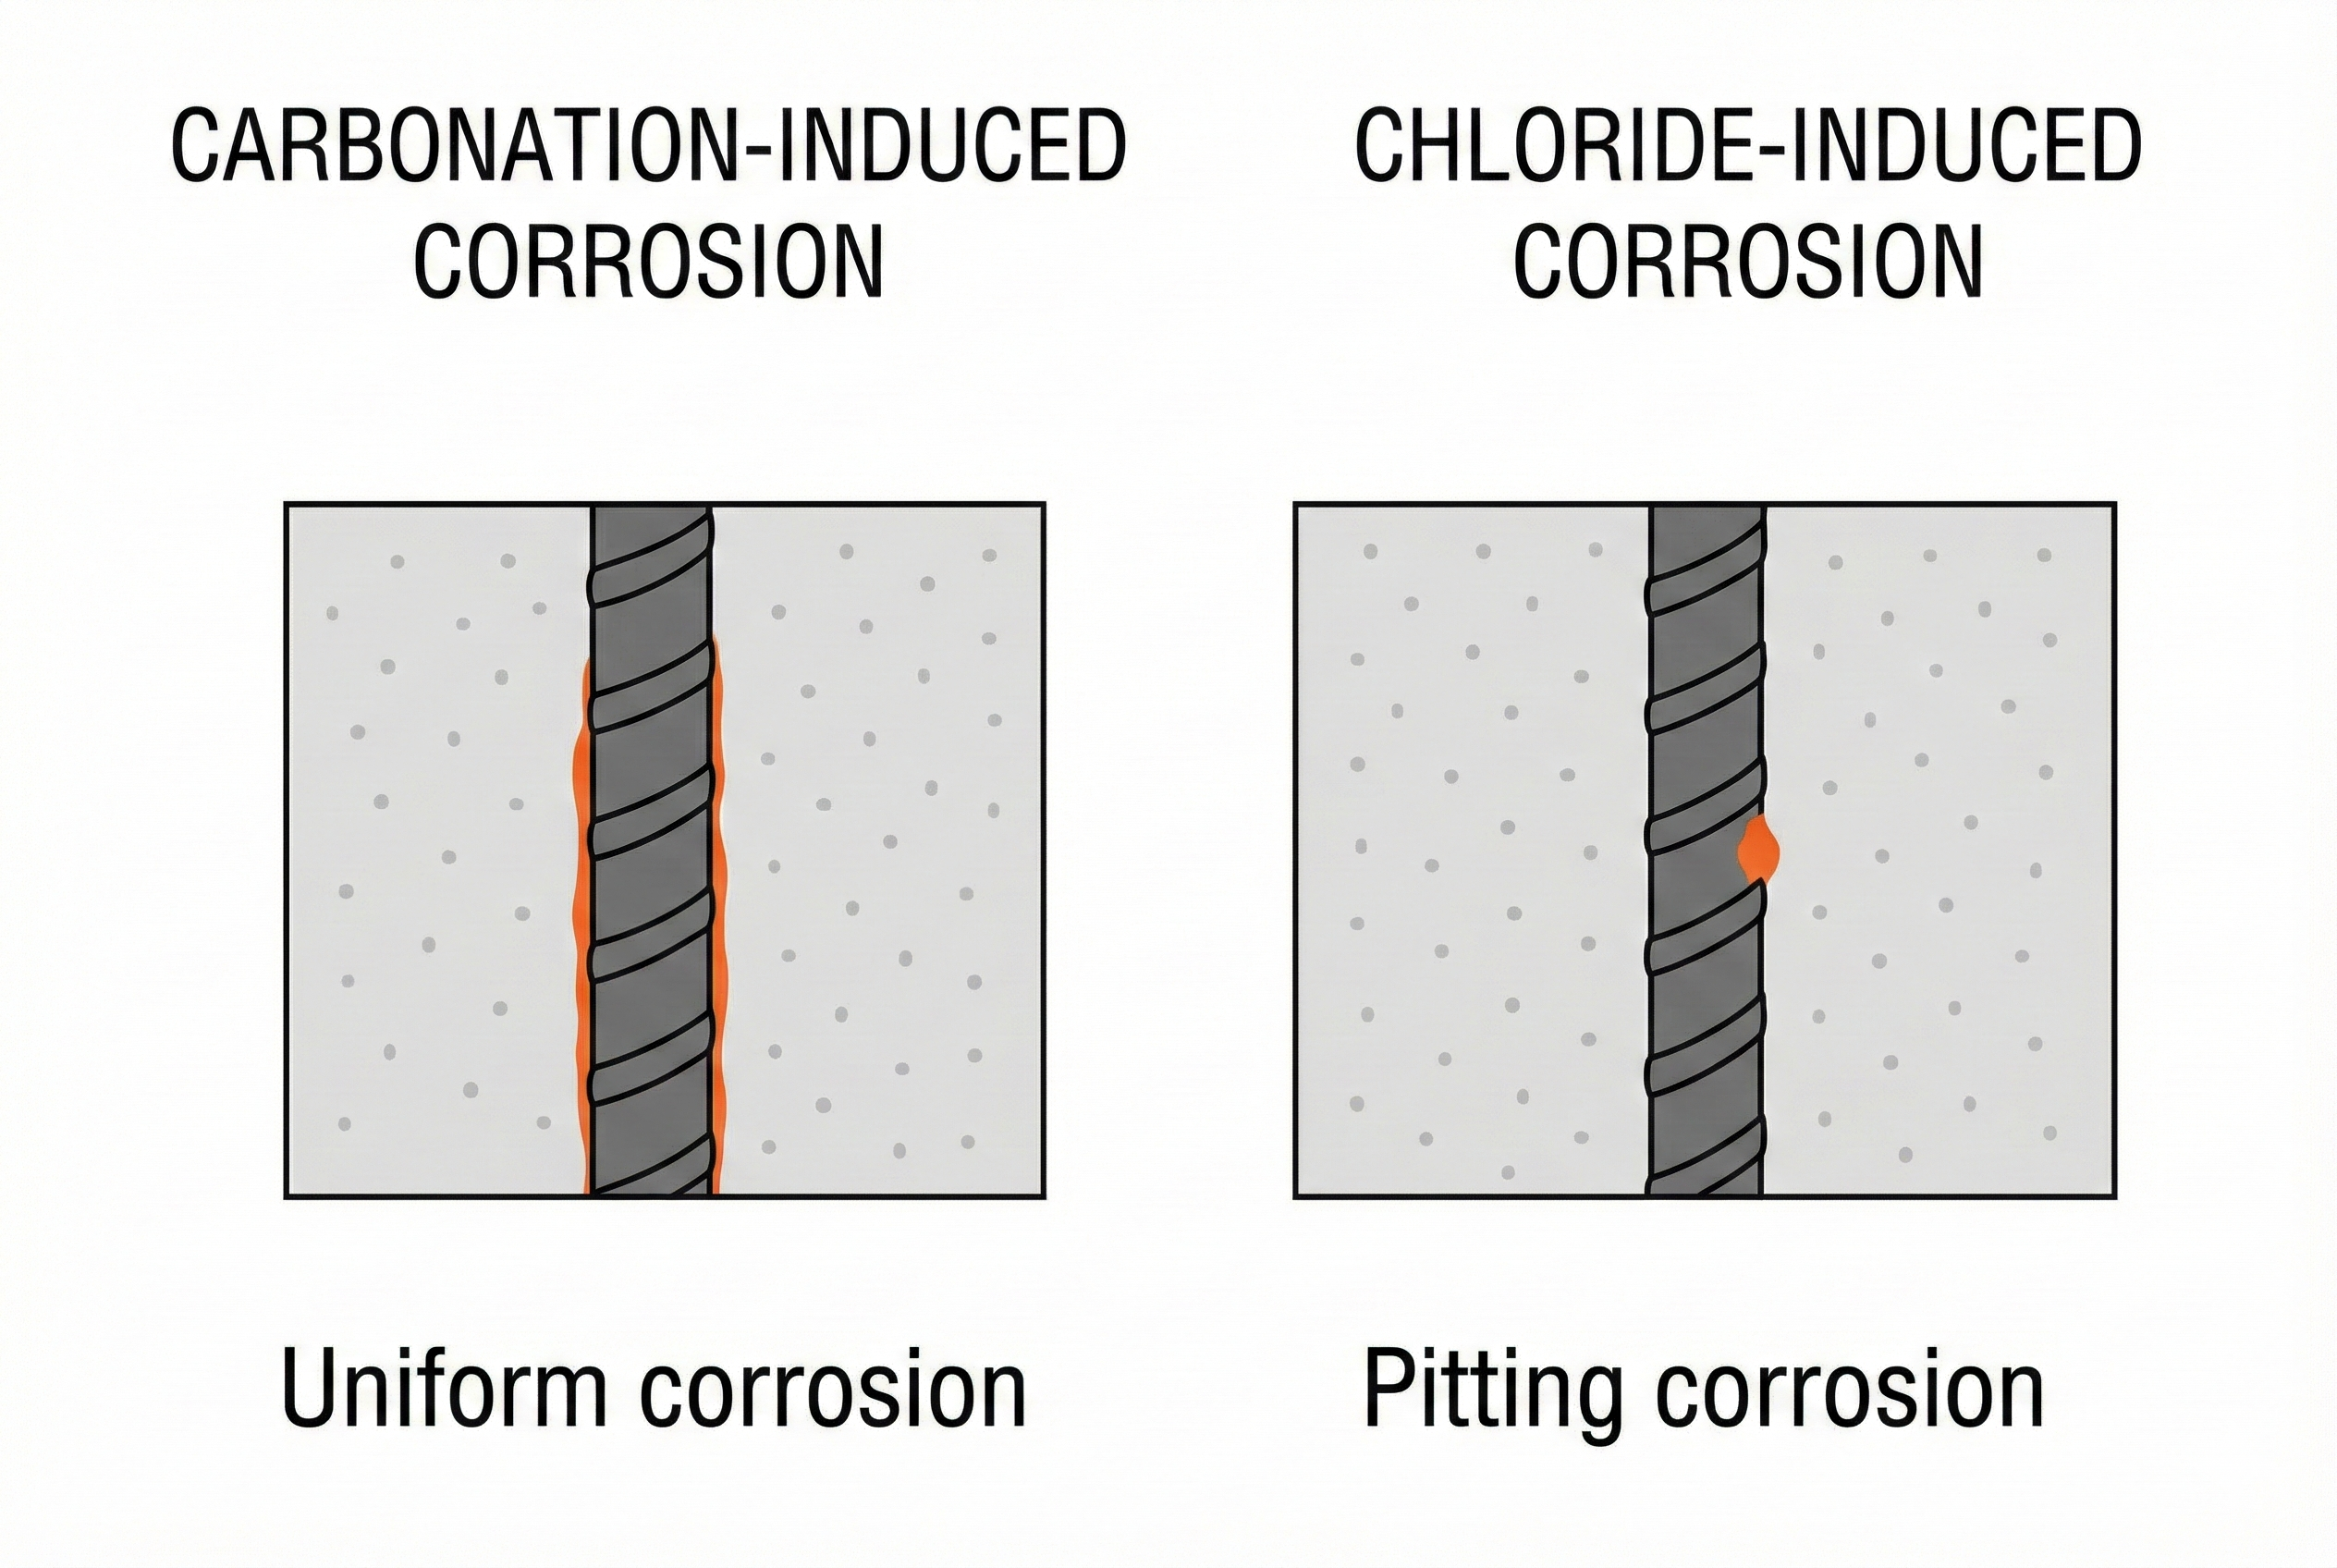
\includegraphics[width=0.5\linewidth]{z_corrosion_en.png}
    \caption{Diferenças entre os mecanismos de corrosão localizada (cloretos) e generalizada (carbonatação). \falta{traduzir a figura para o português, se for mantida a versão em inglês indicar na legenda}}
    \label{fig:z_corrosion_en}
\end{figure}

\subsection{Modelo de avanço da frente de carbonatação}
\label{subsec:modelo_possan}

O modelo proposto por \citet{possan2010} oferece uma abordagem paramétrica para a previsão da profundidade de carbonatação $y(t)$ em estruturas de concreto armado, integrando variáveis de material e de ambiente. A formulação matemática, expressa na Equação~\eqref{eq:y}, estima o avanço da frente de carbonatação ao longo do tempo, considerando a influência da resistência à compressão ($f_c$), do tipo de cimento, das adições minerais, da concentração de CO$_2$ e da umidade relativa ($UR$):

\begin{equation}\label{eq:y}
y(t) = k_c \cdot \left( \frac{20}{f_c} \right)^{k_{fc}} \cdot \left( \frac{t}{20} \right)^{\frac{1}{2}} \cdot \exp \left[ \frac{k_{ad} \cdot ad^{\frac{3}{2}}}{40 + f_c} + \frac{k_{CO_2} \cdot CO_2^{\frac{1}{2}}}{60 + f_c} - \frac{k_{UR} \cdot (UR - 0{,}58)^2}{100 + f_c} \right] \cdot k_{ce}
\end{equation}

\noindent em que $k_c$, $k_{fc}$, $k_{ad}$, $k_{CO_2}$, $k_{UR}$ e $k_{ce}$ são coeficientes calibrados em função do tipo de cimento e da condição de exposição, $ad$ é o teor de adições e $t$ é o tempo de exposição em anos. Em formulações simplificadas, frequentemente utilizadas em análises de confiabilidade, o avanço da frente reduz-se à clássica lei da raiz do tempo,

\begin{equation}\label{eq:raiz_t}
y_{\mathrm{carb}}(t) = k\,\sqrt{t},
\end{equation}

\noindent na qual o coeficiente de carbonatação $k$ (mm/$\sqrt{\text{ano}}$) condensa o efeito conjunto de material e ambiente, podendo ser obtido por regressão de perfis medidos como $k = y/\sqrt{t}$.

A despassivação ocorre quando a frente de carbonatação atinge o nível da armadura, isto é, quando $y_{\mathrm{carb}}(t) \geq c_{\mathrm{nom}}$, em que $c_{\mathrm{nom}}$ é o cobrimento nominal. O instante de iniciação da corrosão, $t_{\mathrm{ini}}$, é definido como a primeira raiz dessa condição. A partir desse ponto inicia-se a fase de propagação, tratada na Seção~\ref{sec:resist}.

\subsection{Base de dados e perfis de referência}
\label{subsec:dataset}

Para a caracterização probabilística do fenômeno, este estudo apoia-se em uma base de dados abrangente de progressão da carbonatação em estruturas de concreto, composta por 20.000 amostras, obtida em trabalho anterior do grupo \citep{couto2025}. A base incorpora variáveis numéricas e categóricas que caracterizam as condições ambientais, as propriedades dos materiais e os fatores temporais que influenciam a profundidade de carbonatação: concentração atmosférica de CO$_2$ (\%), resistência à compressão aos 28 dias $f_c$ (MPa), umidade relativa $UR$ (\%), tempo de exposição $t$ (anos), tipo de cimento (seis classes segundo a \citet{nbr16697}: CP~V-ARI, CP~II-E, CP~II-F, CP~II-Z, CP~III e CP~IV) e condição de exposição (interna protegida, externa protegida e externa desprotegida). A variável-alvo é a profundidade de carbonatação $y$ (mm). A Tabela~\ref{tab:statistics} apresenta as estatísticas descritivas das variáveis numéricas.

\begin{table}[htpb!]
    \centering
    \small
    \caption{Estatísticas descritivas das variáveis numéricas da base de dados de carbonatação ($n = 20.000$) \citep{couto2025}.}
    \label{tab:statistics}
     \begin{tabular}{lrrrr}
    \toprule
     & \textbf{média} & \textbf{desvio} & \textbf{mín.} & \textbf{máx.} \\
    \midrule
    \textbf{CO$_2$ (\%)} & 0,16 & 0,08 & 0,03 & 0,30 \\
    \textbf{$f_c$ (MPa)} & 34,90 & 8,66 & 20,00 & 50,00 \\
    \textbf{$UR$ (\%)} & 59,94 & 17,31 & 30,00 & 90,00 \\
    \textbf{$t$ (anos)} & 49,93 & 29,32 & 0,00 & 100,00 \\
    \textbf{prof. carbonatação (mm)} & 16,59 & 12,84 & 0,00 & 119,71 \\
    \bottomrule
    \end{tabular}
\end{table}

Em \citet{couto2025}, sete modelos de aprendizado de máquina foram treinados sobre essa base para a predição da profundidade de carbonatação, com validação cruzada de 10 dobras; os modelos de melhor desempenho (rede neural MLP e \textit{Histogram-based Gradient Boosting}) atingiram $R^2 = 0{,}99$ no conjunto de teste, enquanto regressões lineares limitaram-se a $R^2 \approx 0{,}54$, evidenciando a forte não linearidade do fenômeno. Esses resultados validam a base de dados como fonte de perfis representativos de carbonatação e justificam o uso de metamodelos não lineares no presente arcabouço. \falta{se desejado, recuperar aqui a tabela completa de desempenho dos 7 modelos e as figuras de dispersão previsto vs.\ observado do trabalho anterior}

A análise dos perfis de profundidade permitiu determinar coeficientes de carbonatação médios por classe de resistência. Para a condição de exposição interna protegida, que apresentou as maiores taxas de carbonatação, obtiveram-se $k_{20} = 5{,}8$, $k_{30} = 3{,}8$, $k_{40} = 2{,}3$ e $k_{50} = 1{,}7$~mm/$\sqrt{\text{ano}}$ para as classes C20 a C50, respectivamente, conforme ilustrado na Figura~\ref{fig:z_carbonation_profile}.

\begin{figure}[htpb!]
        \centering
        
\includegraphics[width= 0.60\textwidth]{z_carbonation_profile.png}
        \caption{Perfis de carbonatação para exposição interna protegida e coeficientes de carbonatação por classe de resistência. \falta{traduzir rótulos da figura para o português}}
        \label{fig:z_carbonation_profile}
\end{figure}

\subsection{Perfil temporal de CO$_2$ atmosférico}
\label{subsec:co2}

Para modelar a evolução temporal da concentração atmosférica de CO$_2$ --- parâmetro fundamental das simulações de degradação de longo prazo --- adotou-se uma abordagem baseada em registros históricos e instrumentais. Para o período de 1900 a 1950, os dados derivam de registros paleoclimáticos de alta resolução extraídos de testemunhos de gelo antártico (Law Dome), mantidos pelo NOAA/NCEI \citep{noaa_law_dome}. A partir de 1950, o modelo ancora-se em medições atmosféricas diretas e contínuas do observatório de Mauna Loa, mantidas pelo NOAA Global Monitoring Laboratory \citep{noaa_gml}.

Para uso nesta pesquisa, foi ajustada uma regressão analítica por partes que simula esse perfil de acumulação de CO$_2$, com coeficiente de determinação $R^2 = 0{,}99$. O arcabouço matemático divide a série temporal em três regimes contínuos de crescimento antropogênico, ilustrados na Figura~\ref{fig:evolution_co2}: crescimento linear lento entre 1900 e 1950, crescimento linear acelerado entre 1950 e 2000 e crescimento quadrático após 2000, capturando a intensificação contemporânea das emissões globais. \falta{apresentar as equações dos três trechos da regressão por partes}

\begin{figure}[htpb!]
    \centering
    
\includegraphics[width=0.5\linewidth]{z_graph_1900_co2.png}
    \caption{Regressão por partes da concentração atmosférica de CO$_2$ simulada de 1900 a 2150. \falta{traduzir rótulos da figura}}
    \label{fig:evolution_co2}
\end{figure}

Como ilustração da aplicação dos modelos descritos, simulações paramétricas projetaram o avanço da carbonatação para o período estendido de 1900 a 2150. As Figuras~\ref{fig:evolution_fck} e \ref{fig:evolution_h} apresentam a evolução temporal da frente de carbonatação, destacando a influência direta da classe de resistência ($f_{ck}$) e da umidade relativa sobre a taxa de degradação. Para fins de avaliação de vida útil, adotou-se uma linha de referência em 30~mm, correspondente a um cobrimento normativo típico \citep{nbr6118}, indicando o limiar teórico de despassivação da armadura. Observa-se, em particular, a aceleração da degradação em ambientes de umidade intermediária (65\%) em comparação com ambientes mais secos (50\%) ou mais úmidos (80\%).

\begin{figure}[htpb!]
    \centering
    \begin{subfigure}[b]{0.48\textwidth}
        \centering
        
\includegraphics[width=\linewidth]{z_graph_1900_fck.png}
        \caption{Influência da classe de resistência $f_{ck}$ ($UR = 65\%$).}
        \label{fig:evolution_fck}
    \end{subfigure}
    \hfill
    \begin{subfigure}[b]{0.48\textwidth}
        \centering
        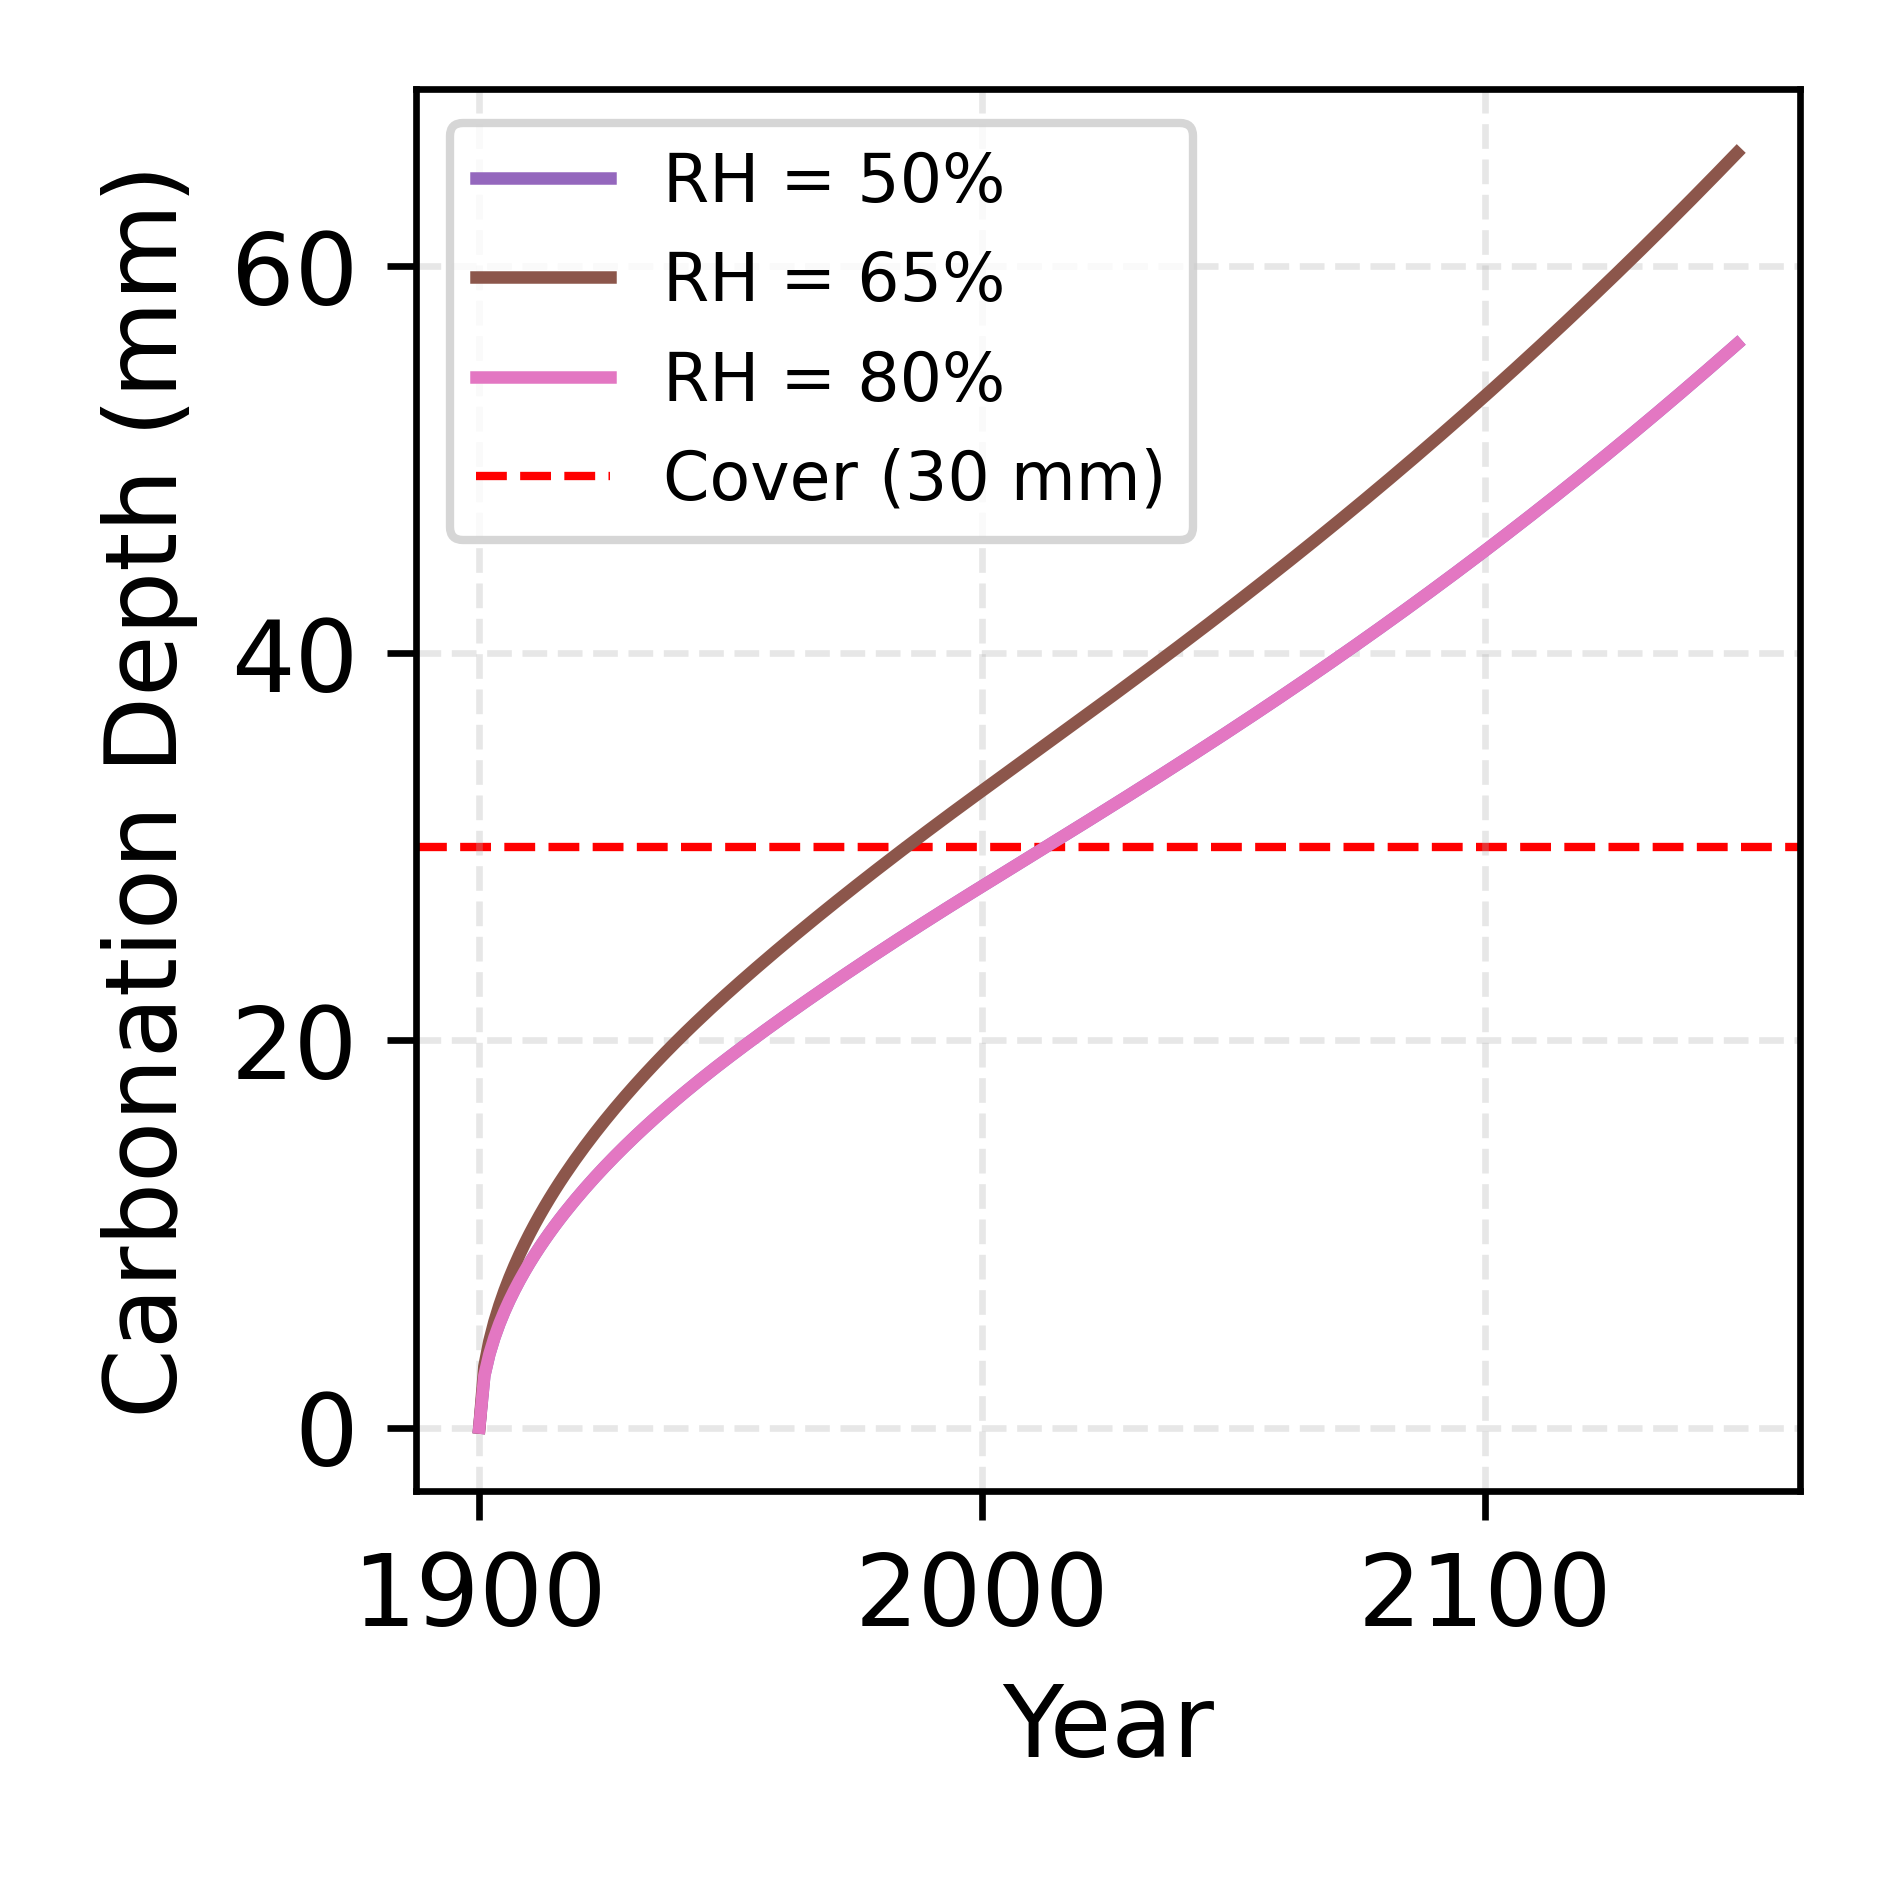
\includegraphics[width=\linewidth]{z_graph_1900_h.png}
        \caption{Influência da umidade relativa ($f_{ck} = 30$~MPa).}
        \label{fig:evolution_h}
    \end{subfigure}
    \caption{Evolução temporal da frente de carbonatação (1900--2150) com linha de referência no cobrimento normativo de 30~mm. \falta{traduzir rótulos das figuras}}
    \label{fig:evolucao_carb}
\end{figure}
